\documentclass[14pt, a4paper]{extarticle}

\usepackage[utf8]{inputenc}
\usepackage[T1]{fontenc}
\usepackage{amsmath}
\usepackage{amssymb}
\usepackage{graphicx}
\usepackage[left=2.00cm, right=2.00cm, top=2.00cm, bottom=2.00cm]{geometry}
\usepackage[russian]{babel}

\usepackage{setspace}
\usepackage{fancyhdr}

\graphicspath{{img/}}

\RequirePackage{caption}
\captionsetup[figure]{justification=centering,name=Рисунок,labelsep=endash}

\usepackage{indentfirst}

\usepackage{float}

\begin{document}
	\onehalfspacing
	\begin{titlepage}
	\begin{center}
		\begin{small}
			\textbf{Министерство науки и высшего образования Российской Федерации}

			ФЕДЕРАЛЬНОЕ ГОСУДАРСТВЕННОЕ АВТОНОМНОЕ ОБРАЗОВАТЕЛЬНОЕ УЧРЕЖДЕНИЕ ВЫСШЕГО ОБРАЗОВАНИЯ
			
			\textbf{<<НАЦИОНАЛЬНЫЙ ИССЛЕДОВАТЕЛЬСКИЙ УНИВЕРСИТЕТ ИТМО>>}
		\end{small}
		
		\vspace{8em}
		
		Отчет по лабораторной работе №4
		
		СИНТЕЗ ОПТИМАЛЬНОГО УПРАВЛЕНИЯ. ПРИНЦИП МАКСИМУМА
		
		По дисциплине <<Оптимальное управление>>
	\end{center}
	
	\vspace{8em}
	
	\begin{flushright}
		Выполнил:\\
		студент группы R42331c\\
		Манахов~С.П.
		
		\vspace{1em}
		
		Преподаватель:\\
		Парамонов~А.В.
	\end{flushright}

	\vfill
	
	\begin{center}
		\small
		Санкт-Петербург\\
		2022 г.\\
	\end{center}
\end{titlepage}
	\setcounter{page}{2}
	
	\section*{Задание}
	
	\begin{enumerate}
		\item Дан возмущённый линейный объект управления:
		$$\dot{x}=Ax+Bu+B_ff,x(0)$$
		Построить $H_\infty$-оптимальный регулятор вида $u=Kx$. Расчет произвести на основе уравнения Риккати:
		$$A^TP+PA+Q-PBB^TP+\gamma^{-2}PB_fB_f^TP=0$$
		$$K=-B^TP$$
		\item Экспериментально определить минимальное значение коэффициента $\gamma=\gamma_{min}$, при котором существует положительно полуопределённая матрица $P$ в качестве решения уравнения Риккати;
		\item Начальные условия выбрать $x(0)=[1,0]^T$, возмущение $f=10sin6t+5cos2t+4cos3t+3cos8t$;
		\item Для $\gamma_{min}$ построить графики управления $u$ и переменных состояния $x_1$, $x_2$.
		\item Определить $H_\infty$-нормы передаточных функций $C_1(Is-(A+BK))^{-1}B_f$ и $C_2(Is-(A+BK))^{-1}B_f$, где $C_1=\left[\begin{matrix}1 & 0\end{matrix}\right]$ и $C_2=\left[\begin{matrix}0 & 1\end{matrix}\right]$;
		\item Определить $H_\infty$-норму передаточной функции $(Is-(A+BK))^{-1}B_f$.
	\end{enumerate}
	\begin{table}[H]
		\centering
		\begin{tabular}{|c|c|c|c|c|}
			\hline
			Вариант & $A$ & $B$ & $B_f$ & $Q$ \\\hline
			9 & 
			$\left[\begin{matrix}
				2 & 3 \\
				6 & 0 \\
			\end{matrix}\right]$ & 
			$\left[\begin{matrix}
				0 \\ 5 \\
			\end{matrix}\right]$ &
			$\left[\begin{matrix}
				2 \\ 5 \\
			\end{matrix}\right]$ & 
			$\left[\begin{matrix}
				5 & 0 \\
				0 & 5 \\
			\end{matrix}\right]$ \\\hline
		\end{tabular}
	\end{table}
	
	\newpage
	
	\section*{Описание работы}
	
	Полученная при помощи пакета \textit{MATLAB~Simulink} система представлена на рисунках \ref{fig:system}--\ref{fig:properties}.
	
	\begin{figure}[H]
		\centering
		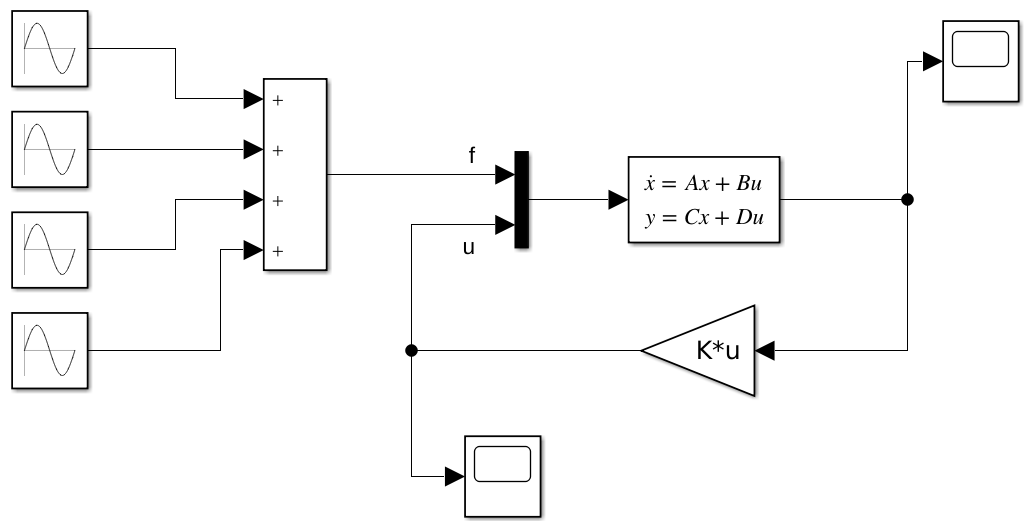
\includegraphics[width=0.6\textwidth]{system}
		\caption{Замкнутая система}
		\label{fig:system}
	\end{figure}
	
	\begin{figure}[H]
		\centering
		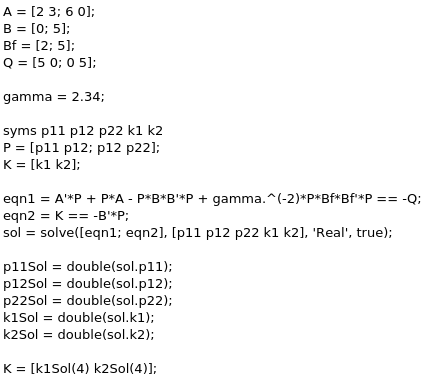
\includegraphics{properties}
		\caption{Параметры системы}
		\label{fig:properties}
	\end{figure}
	
	Полученное экспериментально минимальное значение коэффицента $\gamma=\gamma_{min}=2,34$.
	
	Промоделируем полученную систему при $x(0)=[1,0]^T$, $f=10sin6t+5cos2t+4cos3t+3cos8t$. Полученные графики представлены на рисунках \ref{fig:x-4},\ref{fig:u-4}.
	
	\begin{figure}[H]
		\centering
		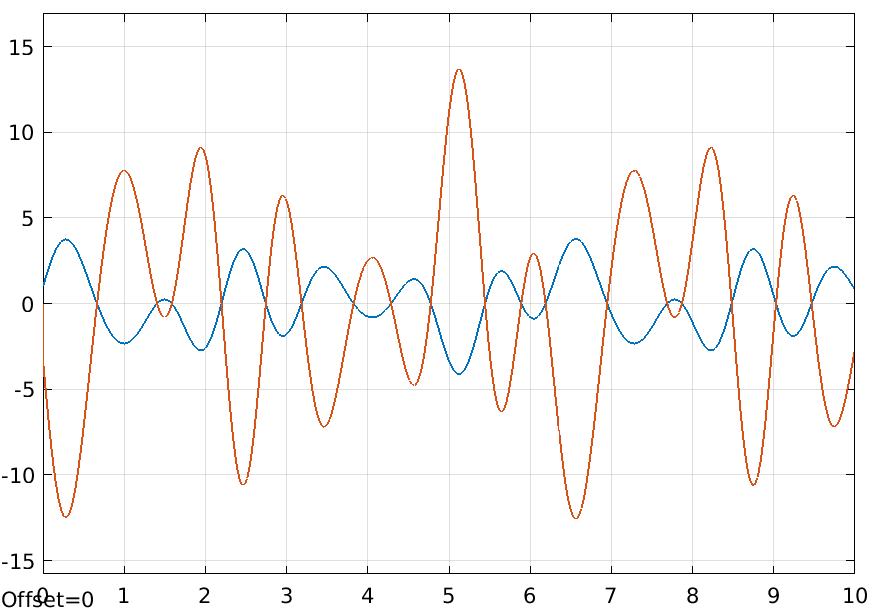
\includegraphics[width=0.6\textwidth]{x-4}
		\caption{Вектор состояния системы $x$}
		\label{fig:x-4}
	\end{figure}
	
	\begin{figure}[H]
		\centering
		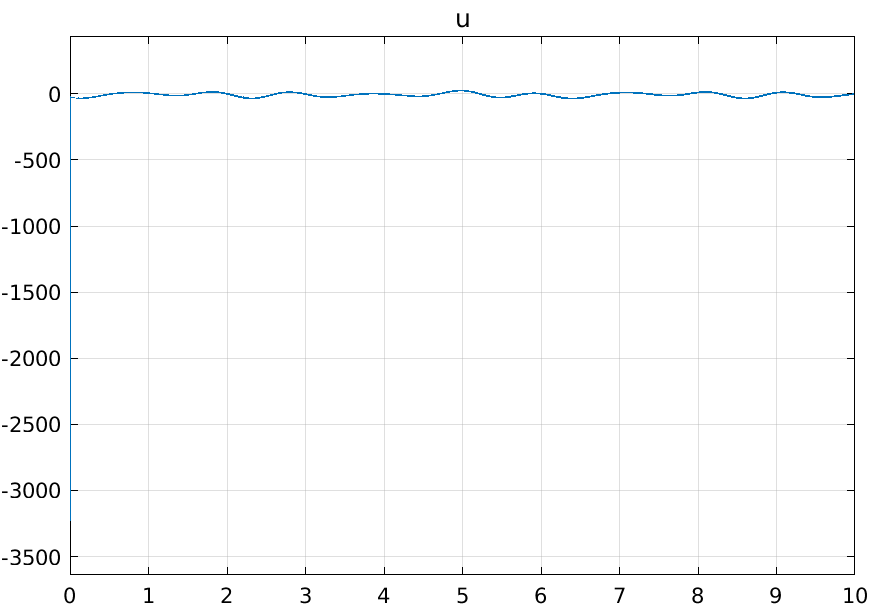
\includegraphics[width=0.6\textwidth]{u-4}
		\caption{Управляющий сигнал системы $u$}
		\label{fig:u-4}
	\end{figure}
	
	$H_\infty$-нормы передаточных функций $C_1(Is-(A+BK))^{-1}B_f$ и $C_2(Is-(A+BK))^{-1}B_f$ при $C_1=\left[\begin{matrix}1 & 0\end{matrix}\right]$ и $C_2=\left[\begin{matrix}0 & 1\end{matrix}\right]$ соответственно равны:
	$$\begin{matrix}
		\left|\left|W\right|\right|_{\infty1} = 0,2501; & \left|\left|W\right|\right|_{\infty2} = 0,8334 \\
	\end{matrix}$$
	
	$H_\infty$-норма передаточной функции $(Is-(A+BK))^{-1}B_f$ равна:
	$$\left|\left|W\right|\right|_\infty=0,8701$$
	
	\newpage
	
	\section*{Вывод}
	
	Построенный в работе при помощи экспериментального определения минимального значения коэффициента $\gamma=\gamma_{min}$ регулятор соответствует наименьшей $H_\infty$-норме передаточной функции системы, что означает наименьшую максимальную амплитуду колебаний системы.

\end{document}